\chapter{8.\hspace{0.5em}Woche}\label{wo8}

\section{Prototype}\label{wo8_1}

\begin{enumerate}[label={\Roman*)}]
	\item Da der letzte von mir gebackene Kuchen sehr gut ankam, entschied ich mich dazu diese Woche wieder einen f\"ur das
Team zu machen, auch um es f\"ur die sehr guten Leistungen des Teams, die sehr zeitaufwendig bearbeitet und abgeschlossen wurden,
trotz immer wieder auftretender Probleme, die, die eigentlich simplen, Aufgaben sehr komplizieren.
	\item Dieses mal entschied ich mich dazu eine Cremetorte zu machen, eigentlich soll es ein K\"asekuchen sein, jedoch
wurde es diesmal eher cremig, wie folgend zu sehen.
\begin{center}
	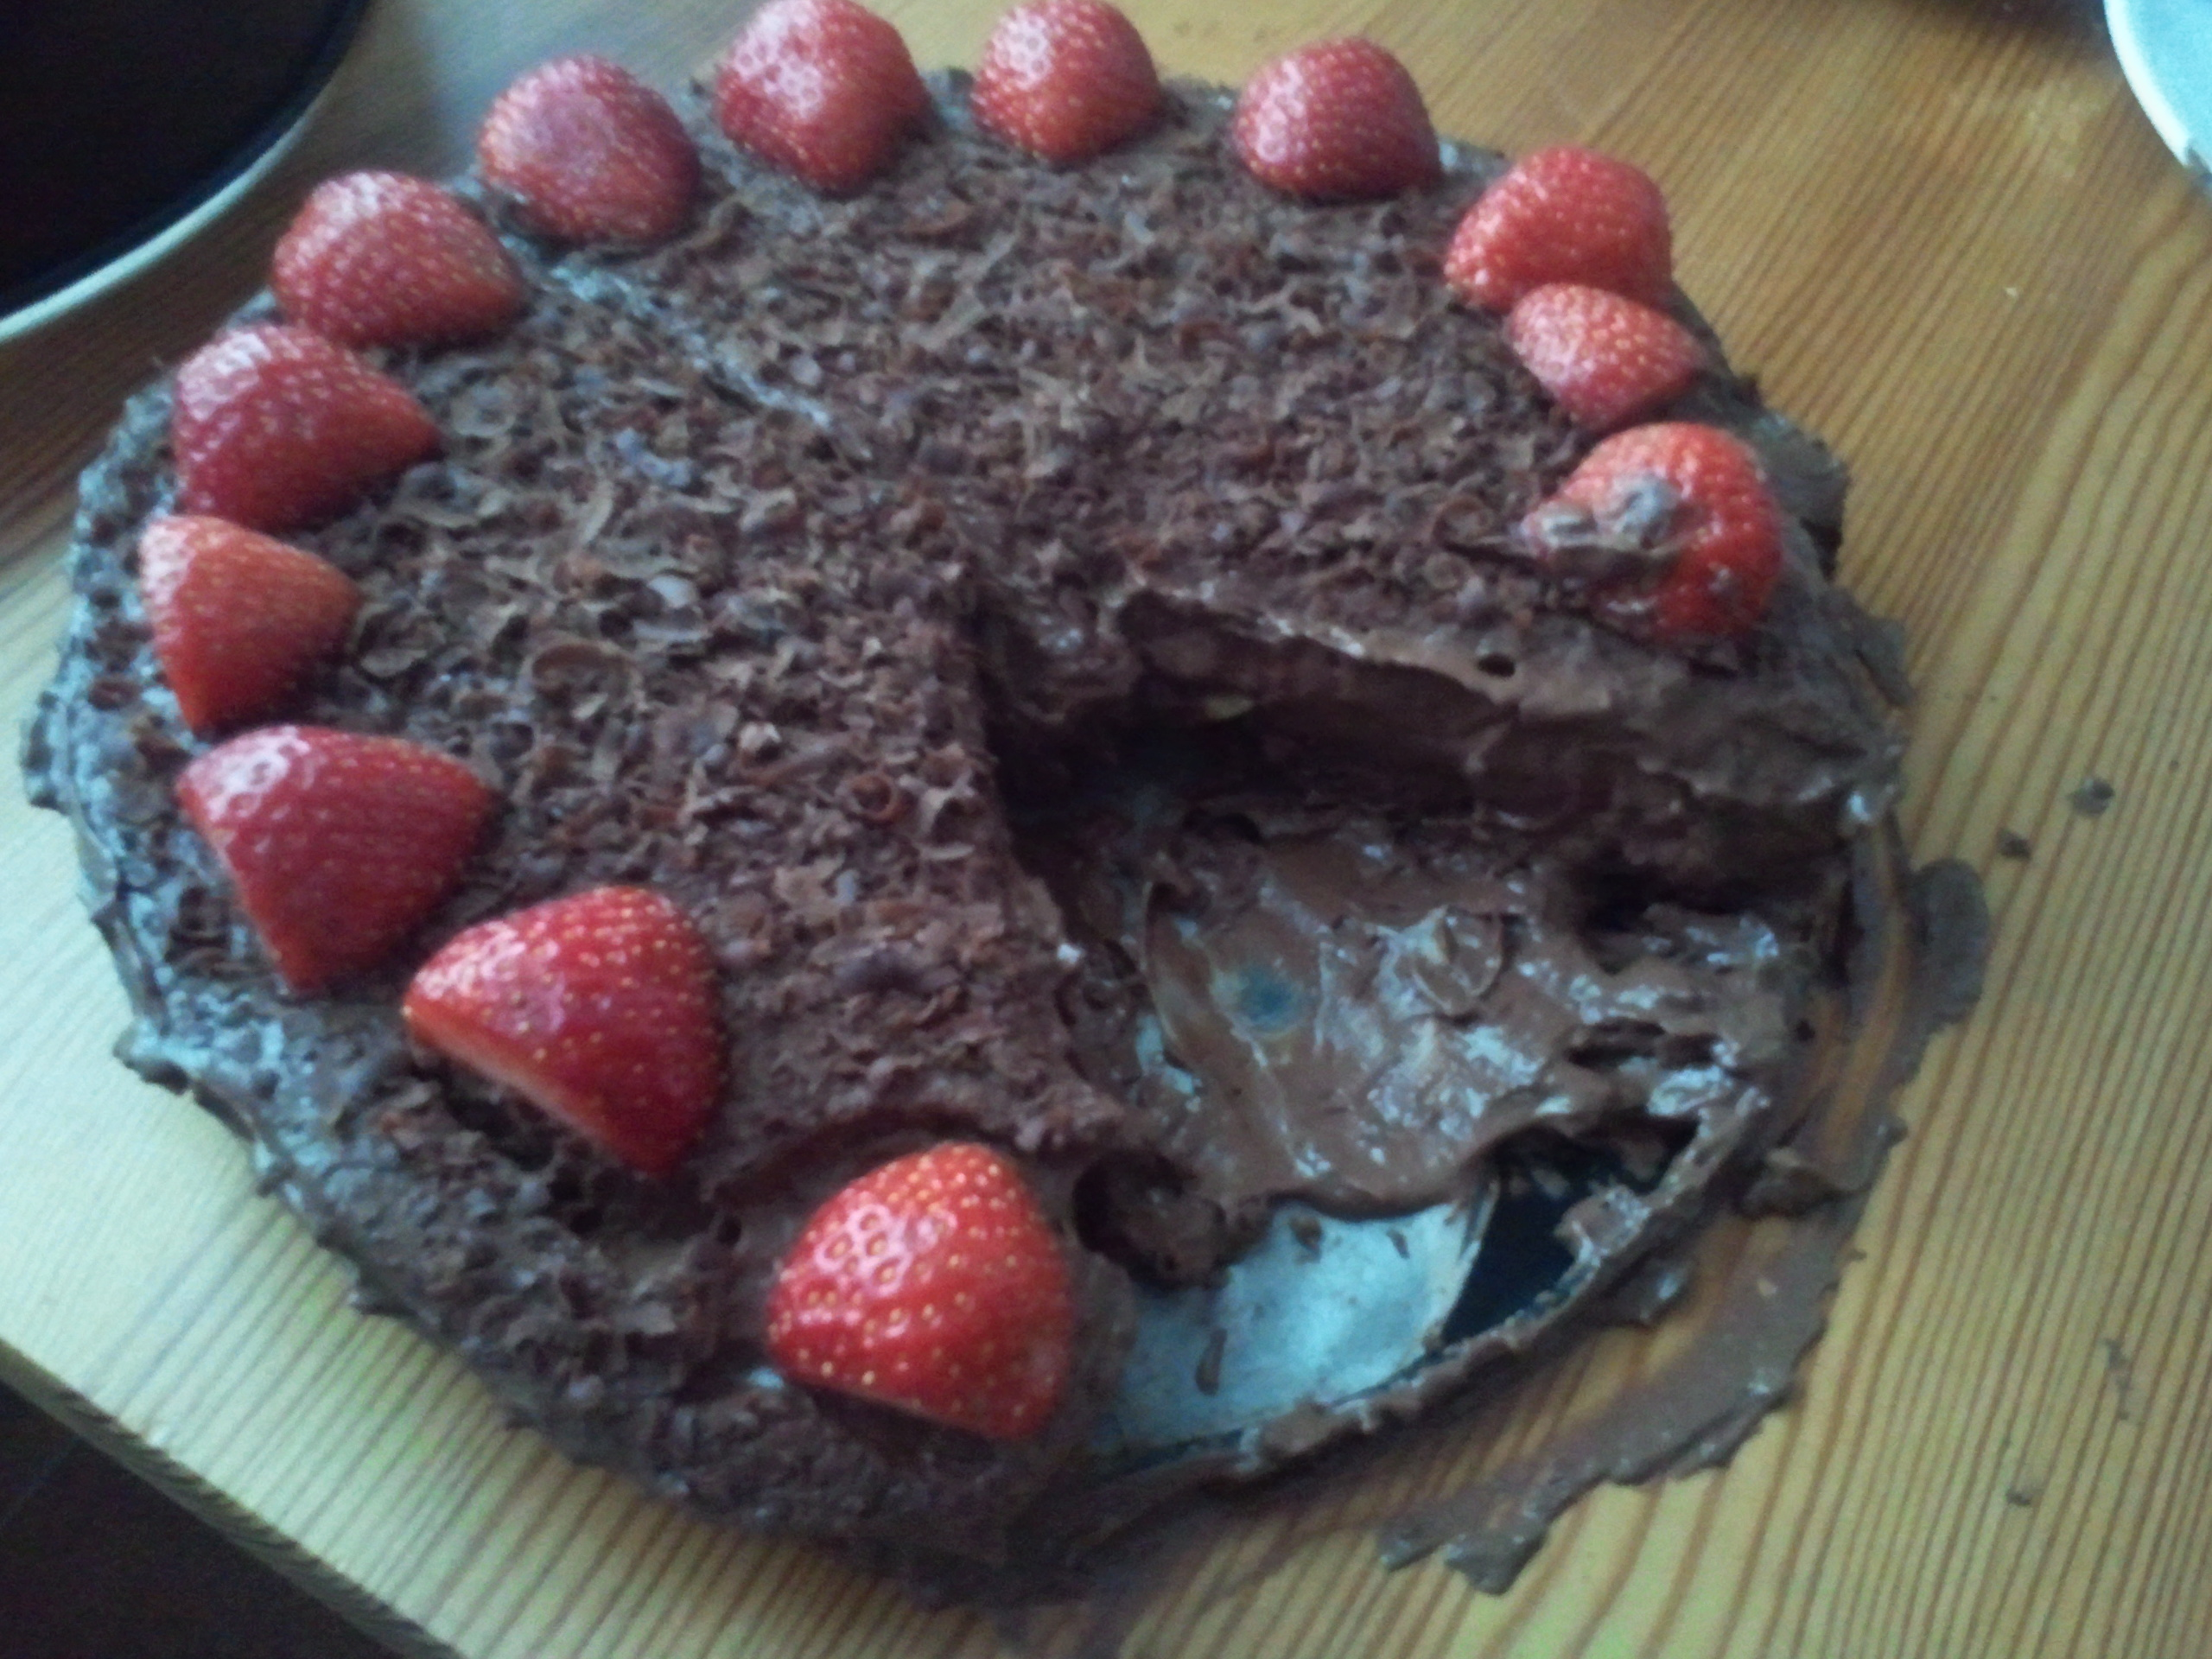
\includegraphics[width=17cm]{img/2012-06-07_10-44-10}
\end{center}
	\item In dieser Woche habe ich die bereits bestehende und funktionierende Funktion der E-Mailversendung weiter ausgebaut
und den gestiegenen Anwendungsf\"allen angepasst.
	\item Weiterhin habe ich mich mit dem Team um die Zuteilung der neuen Aufgaben gek\"ummert, sodass jeder seine zu
bearbeitenden Aufgaben hat und wei\ss{} was zu tun ist.
	\item Mir wurden als neue Aufgaben die Ermittlung der favorisiten aus den bestehenden Touren und das Ermitteln der
initialen Templates f\"ur Touren zugewiesen.
	\item Damit ich meine Aufgaben m\"oglichst zeitnah erledigen kann und es nicht wieder auf den letzten Dr\"ucker
geschieht, wie in der Vergangenheit leider manchmal passiert, habe ich angefangen mich mit dem Thema des Caching intensiv zu
besch\"aftigen und schon im Zusammenhang mit Scala geguckt was dort m\"oglich ist.
	\item Am Freitag haben wir uns in der Universit\"at getroffen und es wurde spontan entschieden, dass Treffen nach
drau\ss{}en auf die Wiese zu verlegen. Dies erheiterte die Stimmung des Treffens, was dem gesamten Verlauf sehr gut entsprach, da
dieses Treffen sehr locker aufgebaut war und es nur um den aktuellen Stand der Gruppen ging, somit war dieses Treffen
allgemein entspannend aufgebaut und verlief sehr angenehm, dies empfand ich als besonders wohltuend f\"ur den allgemeinen Ablauf
des Projektes, da es so nicht zu sehr zu einer enormen Programmieraufgabe wird bei der am Ende ein fertiges Projekt erwartet wird
und nicht auf die Bed\"urfnisse der Studierenden eingegangen wird.
	\item Diese Woche habe ich mich mit dem Team 4 in Verbindung gesetzt, um eine m\"ogliche Zusammenarbeit bereits vor Ende
des Projektes zu erm\"oglichen. Dabei ist geplant, dass von Seiten des Teams 4 aus bei uns automatisch Touren generiert werden,
wenn dort bei einer Planung einer Reise eine Taxifahrt enthalten ist.
\end{enumerate}